\documentclass{iutbscthesis}
\usepackage{longtable,tabularx,enumitem,xcolor,microtype,placeins,url}
\graphicspath{{../assets/}{assets/}}
\addbibresource{citations.bib}
\definecolor{deepblue}{HTML}{173B68}\definecolor{softblue}{HTML}{EAF2FB}\definecolor{softgray}{HTML}{F4F6F8}
\hypersetup{colorlinks=true,linkcolor=deepblue,citecolor=deepblue,urlcolor=deepblue}
\setlist[itemize]{leftmargin=1.8em,itemsep=.2em}\setlist[enumerate]{leftmargin=1.8em,itemsep=.2em}
\lstset{basicstyle=\ttfamily\small,breaklines=true,frame=single,backgroundcolor=\color{softgray},showstringspaces=false}
\title{A Controlled Comparison of Flow Matching and Mean Flow for Unconditional CIFAR-10 Image Generation}
\addauthor{Sheikh Mosheul Akbar}{220041137}
\addauthor{Md. Samiul Islam}{220041027}
\addauthor{Rad Shahmad Daiyan}{220041209}
\supervisor{Dr. Md. Azam Hossain}{Supervisor}{Department of Computer Science and Engineering}
\addcosupervisor{Samnun Azfar}{Co-Supervisor}{Department of Computer Science and Engineering}
\department{Department of Computer Science and Engineering}
\program{BACHELOR OF SCIENCE IN COMPUTER SCIENCE AND ENGINEERING}
\defensedate{14}{September}{2026}
\begin{document}
\pagenumbering{roman}\titlepage
\chapter*{Declaration}\addcontentsline{toc}{chapter}{Declaration}
We declare that this report is an original account of the submitted system and experiments. External ideas, datasets, and metrics are cited. Numerical claims are derived from the supplied JSONL logs under the audit rule in Section~\ref{sec:audit}. All visibly marked repository, meeting, contribution, and future-work placeholders must be completed before physical submission.
\par\vspace{2cm}
\noindent\begin{tabularx}{\textwidth}{X p{.30\textwidth}}
Sheikh Mosheul Akbar: \hrulefill & Date: \hrulefill\\[2em]
Md. Samiul Islam: \hrulefill & Date: \hrulefill\\[2em]
Rad Shahmad Daiyan: \hrulefill & Date: \hrulefill
\end{tabularx}
\clearpage
\chapter*{Acknowledgement}\addcontentsline{toc}{chapter}{Acknowledgement}
We express our sincere gratitude to our supervisor, Dr. Md. Azam Hossain, and our co-supervisor, Samnun Azfar, for their guidance, critical feedback, and encouragement throughout this design project. We also thank the Department of Computer Science and Engineering and the computing facilities that supported the training and evaluation runs. Finally, we acknowledge the researchers and open-source communities behind Flow Matching, Mean Flow, CIFAR-10, PyTorch, and TorchMetrics, whose published work and software made this comparative study possible.
\clearpage
\begin{abstract}
This project studies how the target learned by a continuous-time generator and the distribution used to sample training time affect image quality and inference cost. Three unconditional CIFAR-10 systems are implemented in one algorithm-agnostic pipeline: Flow Matching (FM) with uniform time, FM with logit-normal time, and Mean Flow (MF) with interval-conditioned average velocity. All use one 6,352,899-parameter time-conditioned SimpleUNet; MF adds 323 parameters for the second interval endpoint. The system records loss, synchronized timing, memory, checkpoints, sample grids, Frechet Inception Distance (FID), and Inception Score (IS), and exposes trained checkpoints through interactive history and inference views.

The strongest submitted configuration is logit-normal FM at 20 function evaluations (NFE), with FID 72.66 and IS $6.18\pm0.52$ on 1,000 samples. Standard FM reaches FID 76.10 and IS $6.12\pm0.72$. MF gives the best one-step result of the three runs (FID 210.99; IS $2.54\pm0.21$), but its loss rises over 30 epochs and more NFEs do not improve quality. Thus, under these budgets, logit-normal FM is the strongest multi-step system, while MF needs further optimization before its intended one-step benefit becomes competitive. Because batch size, epochs, learning rate, hardware context, and sample count are not fully matched, results are reported as audited engineering evidence rather than a universal ranking.
\end{abstract}
\tableofcontents\listoffigures\listoftables\clearpage
\begin{abbreviations}
\abbr{AMP}{Automatic Mixed Precision}\abbr{CFM}{Conditional Flow Matching}\abbr{CNF}{Continuous Normalizing Flow}\abbr{FID}{Frechet Inception Distance}\abbr{FM}{Flow Matching}\abbr{IS}{Inception Score}\abbr{JVP}{Jacobian-Vector Product}\abbr{MF}{Mean Flow}\abbr{MSE}{Mean Squared Error}\abbr{NFE}{Number of Function Evaluations}\abbr{ODE}{Ordinary Differential Equation}\abbr{UI}{User Interface}\abbr{VRAM}{Video Random Access Memory}
\end{abbreviations}
\clearpage\pagenumbering{arabic}

\chapter{Introduction}
\section{Motivation}
Continuous-time generators transform a simple noise distribution into an image distribution through a learned trajectory. Repeated network evaluations improve numerical integration but create a quality--latency trade-off. FM trains a vector field for a prescribed probability path without simulating that path during training \cite{lipman2023flow}. MF instead learns average velocity over an interval and aims to make a full noise-to-data displacement possible in one call \cite{geng2025mean}. A third configuration tests logit-normal time sampling, motivated by rectified-flow work that emphasizes perceptually relevant intermediate noise levels \cite{esser2024scaling}.
\section{Problem statement}
Algorithm comparisons become unreliable if the model, preprocessing, evaluator, seed, or log interpretation changes between runs. This project therefore combines implementation with evidence control: all algorithms use shared infrastructure, while every remaining configuration difference and threat to validity is reported.
\section{Aim, objectives, and questions}
The aim is to build and critically evaluate a reproducible educational system for unconditional CIFAR-10 generation. Objectives are to formalize the objectives and samplers; preserve a common backbone; centralize training, checkpointing, timing, and evaluation; measure NFE $\{1,5,10,20\}$; retain epoch evidence; and provide a local live demo.
\begin{description}
\item[RQ1.] How do the three objectives behave during training?
\item[RQ2.] How does sample quality change with NFE?
\item[RQ3.] What quality--latency trade-offs are observed?
\item[RQ4.] Does this MF run realize competitive one-step generation?
\item[RQ5.] Can claims be traced to configurations, checkpoints, logs, and UI behavior?
\end{description}
\section{Contributions}
The deliverable includes complete FM, logit-normal FM, and MF implementations; a shared 6.35M-parameter backbone; restart-safe checkpoints; structured JSONL evidence; cached real-image references; FID/IS evaluation; synchronized checkpoint/loss playback; a trained-model inference API; and a deterministic duplicate-log audit.

\chapter{Background and Related Work}
\section{Continuous generative flows}
A continuous model parameterizes $dx_t/dt=v_\theta(x_t,t)$. Neural ODEs established a general framework in which a neural network defines this derivative and an ODE solver computes the transformation \cite{chen2018neural}. NFE counts network calls; synchronized wall-clock time is the direct cost measurement.
\section{Flow Matching}
For data $x_0$ and noise $\epsilon\sim\mathcal N(0,I)$, the implementation uses
\begin{equation}x_t=(1-t)x_0+t\epsilon,\qquad v=\epsilon-x_0.\end{equation}
The loss is
\begin{equation}\mathcal L_{FM}=\mathbb E\|v_\theta(x_t,t)-(\epsilon-x_0)\|_2^2.\end{equation}
Sampling starts at $t=1$ and applies uniform backward Euler steps toward $t=0$ \cite{lipman2023flow}. One step can be too coarse when the learned field varies along the path.
\section{Logit-normal time sampling}
The variant draws $u\sim\mathcal N(0,1)$ and $t=\sigma(u)$, concentrating samples around intermediate time. Path, target, backbone, and sampler remain unchanged. The idea follows logit-normal rectified-flow training \cite{esser2024scaling}; however, the submitted batch size differs, so this is not a pure ablation.
\section{Mean Flow}
MF models average velocity $u(z_t,r,t)$ over $[r,t]$ and uses
\begin{equation}z_r=z_t-(t-r)u(z_t,r,t).\end{equation}
Training follows
\begin{equation}u(z_t,r,t)=v(z_t,t)-(t-r)\frac{d}{dt}u(z_t,r,t),\end{equation}
with the total derivative computed by a forward-mode JVP with tangents $(v,0,1)$ for $(z,r,t)$ \cite{geng2025mean}. With probability 0.25, $r=t$, recovering instantaneous velocity. This compact CIFAR-10 implementation is not a reproduction of the paper's large-scale headline result.
\section{Backbone, data, and metrics}
U-Net-style encoders, decoders, and skip connections provide multi-scale processing \cite{ronneberger2015unet}. CIFAR-10 comprises 60,000 $32\times32$ color images in ten classes, conventionally split 50,000/10,000 \cite{krizhevsky2009learning}. FID compares real and generated feature statistics \cite{heusel2017gans}; IS rewards confident and diverse classifier predictions \cite{salimans2016improved}. Neither is a complete perceptual test, and 1,000-sample estimates should not be compared directly to standard 50,000-sample benchmarks.

\chapter{Problem Definition, Scope, and Validity}
\section{Boundary}
Scope includes unconditional $32\times32$ RGB generation, data loading, shared model construction, three algorithm classes, training, checkpoints, sampling, FID/IS, logs, and local demonstration. It excludes class/text conditioning, high resolution, distributed training, human evaluation, and public deployment.
\section{Controlled and uncontrolled factors}
Dataset, normalization, seed, output size, backbone constructor, evaluator, NFE grid, and evaluation count are shared. Objective and time sampling intentionally change. Available runs also differ in batch, epochs, learning rate, loader workers, and execution environment.
\begin{table}[htbp]\centering\caption{Submitted configurations.}\label{tab:config}
\begin{tabular}{lrrrrl}\toprule Run&Epochs&Batch&Learning rate&Seed&Time sampling\\\midrule
FM&100&128&$2\times10^{-4}$&0&Uniform\\
FM + logit-normal&100&32&$2\times10^{-4}$&0&$\sigma(\mathcal N(0,1))$\\
MF&30&32&$5\times10^{-5}$&0&Uniform $t$, $r\le t$\\\bottomrule\end{tabular}\end{table}
The evidence supports conclusions about these artifacts, not universal algorithm superiority. Stronger causal claims require matched budgets, multiple seeds, larger evaluation sets, and ablations.

\chapter{Methodology}\label{chapter:methodology}
\section{Pipeline}
The flow is configuration $\rightarrow$ dataset $\rightarrow$ shared backbone $\rightarrow$ algorithm $\rightarrow$ trainer $\rightarrow$ checkpoint $\rightarrow$ sampler $\rightarrow$ evaluator $\rightarrow$ JSONL/UI. Algorithm files own mathematics; shared modules own experimental controls.
\section{Data}
Images are normalized to $[-1,1]$; generated tensors are clamped to that range before visualization and metrics.
\begin{figure}[htbp]\centering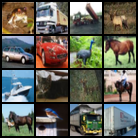
\includegraphics[width=.74\textwidth]{cifar10_examples.png}\caption{Local CIFAR-10 examples enlarged with nearest-neighbor interpolation.}\label{fig:cifar}\end{figure}
\section{Shared backbone}
A 256-D sinusoidal time embedding is transformed by an MLP and injected into residual blocks. The encoder uses base width 64, multipliers $[1,2,2]$, and two blocks per stage; the decoder consumes skips with three blocks per stage. Group normalization and SiLU are used.
\begin{figure}[htbp]\centering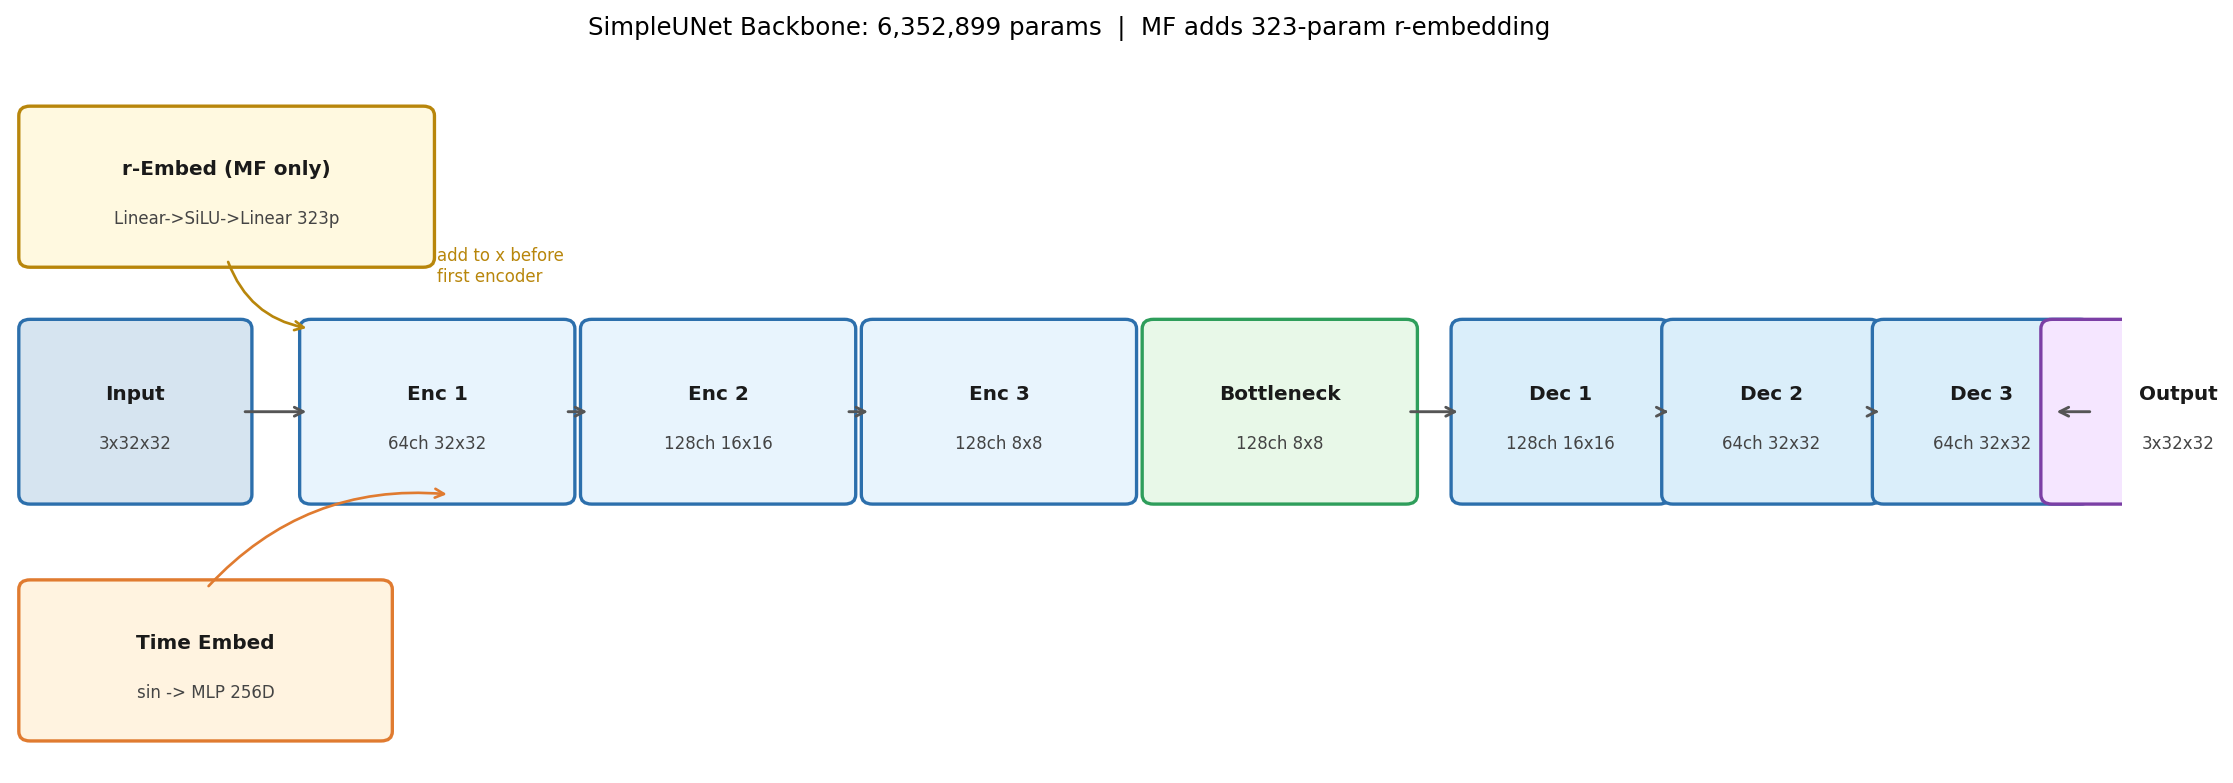
\includegraphics[width=\textwidth]{architecture.png}\caption{Shared SimpleUNet: 6,352,899 parameters. MF adds a separate 323-parameter $r$ embedding.}\label{fig:arch}\end{figure}
MF maps $r$ through Linear$(1,64)$--SiLU--Linear$(64,3)$ and adds the result channel-wise to $z$ before the shared backbone. This is approximately 0.0051\% additional parameters.
\section{Optimization and checkpoints}
All runs use AdamW \cite{loshchilov2019adamw}, zero weight decay, no scheduler, and configured AMP. MF disables autocast inside JVP to avoid mixed-dtype derivative errors. Ten-epoch checkpoints include algorithm, configuration, epoch, module states, optimizer, scheduler, and seed. MF stores both backbone and $r$-embedding states.
\section{Sampling and evaluation}
Each final model produces 1,000 samples at NFE 1, 5, 10, and 20. FM variants apply backward Euler; MF applies one interval displacement per NFE. TorchMetrics receives $[0,255]$ uint8 images in batches of 32. Real tensors are cached and replayed into a fresh FID object for each evaluation, avoiding unreliable caching of internal metric accumulators.
\section{Audit protocol}\label{sec:audit}
Restarts append JSONL rows, causing duplicates. The canonical rule retains the last JSONL occurrence for each epoch and NFE without modifying the source. Checks require valid JSON, unique and contiguous canonical epochs, strictly increasing step/sample counters, finite loss, constant parameters, and complete NFE coverage. All pass. FM repeats epochs 1--10; MF contains earlier attempts and repeats epochs 1--27; logit-normal FM has no duplicate training epochs.

\chapter{Implementation}
\section{Modules and separation of concerns}
\begin{table}[htbp]\centering\caption{Core modules.}\begin{tabularx}{\textwidth}{p{.28\textwidth}X}\toprule
Module&Responsibility\\\midrule
\texttt{config/, data/}&Validated controls and common CIFAR-10 loading\\
\texttt{models/backbone.py}&Time embedding, residual blocks, SimpleUNet\\
\texttt{algorithms/*.py}&Objectives, conditioning, and samplers\\
\texttt{training/, sampling/}&Optimization, timing, checkpoints, generation\\
\texttt{evaluation/}&Common FID/IS implementation\\
\texttt{experiments/runner.py}&End-to-end orchestration and protected controls\\
\texttt{inference\_server.py}&Checkpoint loading and local generation endpoints\\
\texttt{*.html}&Home, synchronized training history, and inference views\\\bottomrule\end{tabularx}\end{table}
Algorithm keyword arguments cannot shadow shared batch, epoch, seed, device, AMP, dataset, backbone, optimizer, evaluation, or output settings.
\section{MF correctness-critical path}
\texttt{torch.func.jvp} receives primals $(z_t,r,t)$ and tangents $(v,0,1)$. The resulting target $v-(t-r)du/dt$ is detached before MSE. The custom embedding is exposed through \texttt{trainable\_modules()}, ensuring optimizer, device, mode, and checkpoint coverage.
\section{UI and inference}
The local service exposes home, training, and inference routes. Inference input is model, NFE, sample count, and seed; output is a generated grid and elapsed time. Training playback maps the slider to saved checkpoint epochs and truncates the loss curve at the same epoch. Epoch 0 is conceptual initial noise; epoch 10 is the first saved trained image.
\section{Reproducibility}
Run-specific configs, metrics, events, grids, checkpoints, and cache metadata are present. The root README still describes algorithm placeholders; executable code and artifacts contradict it. This documentation drift must be corrected before GitHub publication.

\chapter{Results and Discussion}
\section{Training evidence}
\begin{table}[htbp]\centering\caption{Canonical histories.}\label{tab:train}\begin{tabular}{lrrrrrr}\toprule
Run&Epochs&Initial&Final&Steps&Samples&Hours\\\midrule
FM&100&.3201&.1790&39,000&4,992,000&1.75\\
FM + logit-normal&100&.2044&.1414&156,200&4,998,400&3.60\\
MF&30&.5536&.6480&46,860&1,499,520&2.91\\\bottomrule\end{tabular}\end{table}
FM falls 44.1\% and logit-normal FM 30.9\%. MF rises 17.1\%, with its minimum at epoch 1. Objectives differ, so cross-method loss magnitude is not a quality metric; within-run direction is diagnostic.
\begin{figure}[htbp]\centering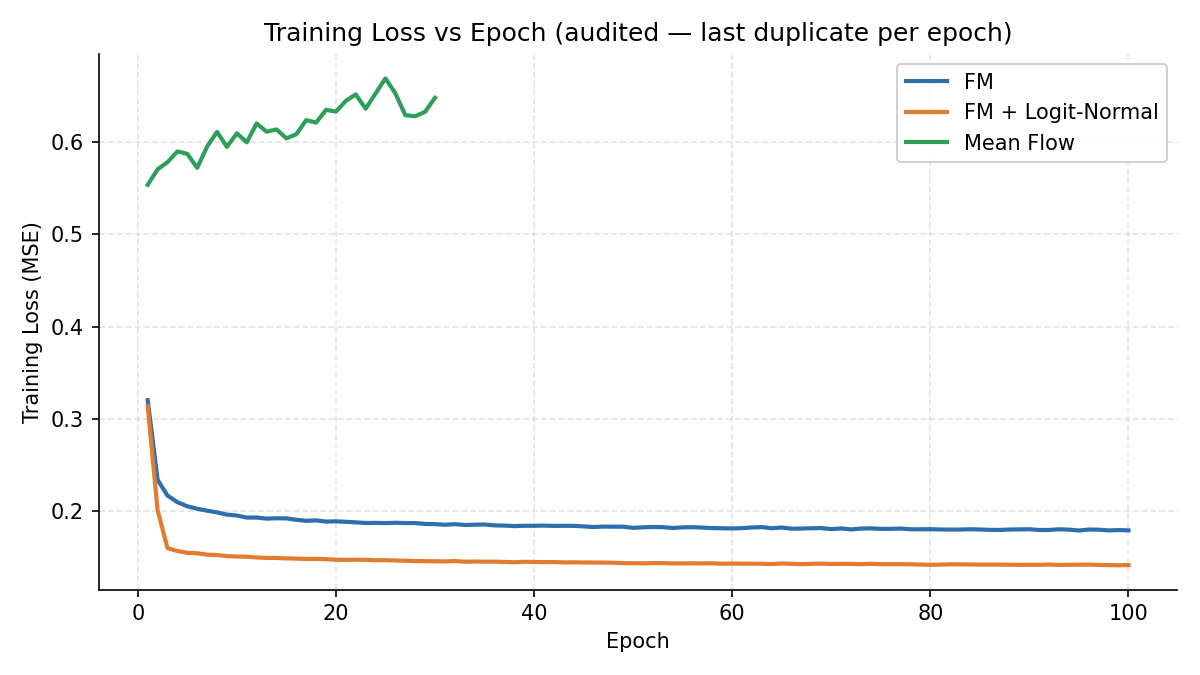
\includegraphics[width=.96\textwidth]{loss_curves.png}\caption{Audited loss histories using the last occurrence of duplicated epochs.}\label{fig:loss}\end{figure}
\section{Quality across inference budgets}
\begin{table}[htbp]\centering\caption{FID and IS on 1,000 generated images.}\label{tab:quality}\begin{tabular}{llrr}\toprule
Run&NFE&FID (lower)&IS (higher)\\\midrule
FM&1&387.81&$1.38\pm.03$\\&5&98.42&$5.21\pm.43$\\&10&81.77&$5.90\pm.53$\\&20&76.10&$6.12\pm.72$\\\midrule
FM + logit-normal&1&362.60&$1.79\pm.05$\\&5&96.45&$5.26\pm.44$\\&10&78.95&$5.93\pm.56$\\&20&\textbf{72.66}&$\mathbf{6.18\pm.52}$\\\midrule
MF&1&210.99&$2.54\pm.21$\\&5&190.12&$2.31\pm.11$\\&10&204.20&$2.18\pm.09$\\&20&214.31&$2.09\pm.09$\\\bottomrule\end{tabular}\end{table}
FM variants improve sharply from 1 to 5 NFE and then gradually. Logit-normal FM leads standard FM at every tested NFE. MF is better than both FM runs at 1 NFE, but its best FID is at 5 and more steps degrade both metrics.
\begin{figure}[htbp]\centering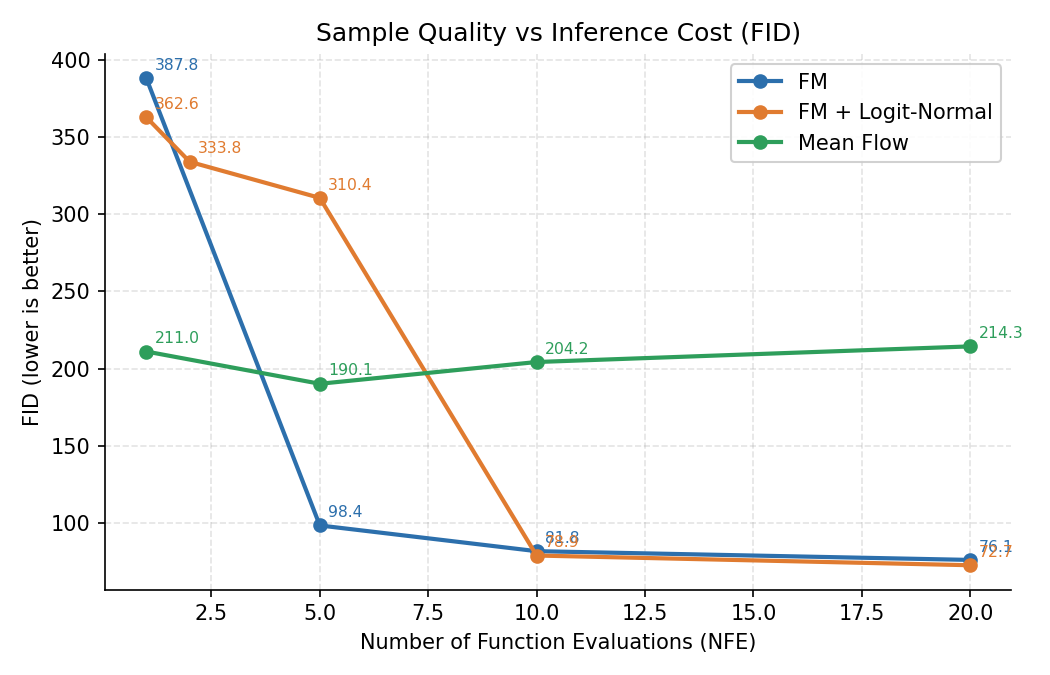
\includegraphics[width=.82\textwidth]{fid_vs_nfe.png}\caption{FID versus NFE.}\label{fig:fid}\end{figure}
\begin{figure}[htbp]\centering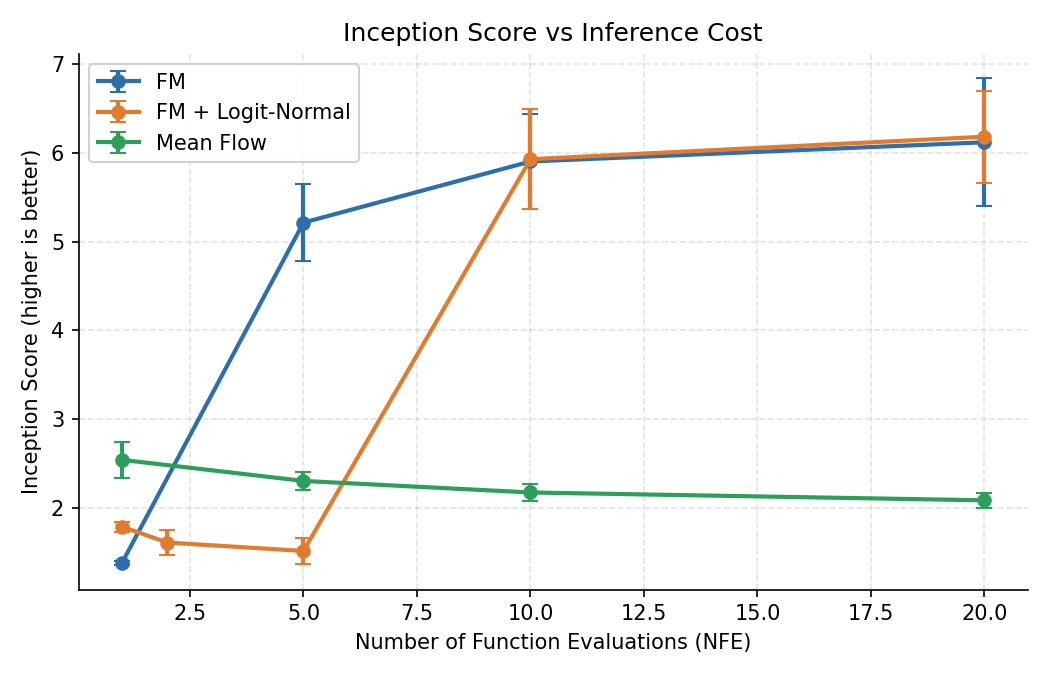
\includegraphics[width=.82\textwidth]{is_vs_nfe.png}\caption{Inception Score versus NFE.}\label{fig:is}\end{figure}
\section{Latency}
Sampling time is approximately linear in NFE. For 1/5/10/20 NFE, logged seconds per 1,000 images are FM: 2.21/12.02/25.07/51.12; logit-normal FM: 0.86/4.88/9.98/19.22; MF: 3.80/13.88/27.77/55.54. Hardware fingerprints are incomplete, so absolute cross-run speed is not an algorithm-only effect.
\begin{figure}[htbp]\centering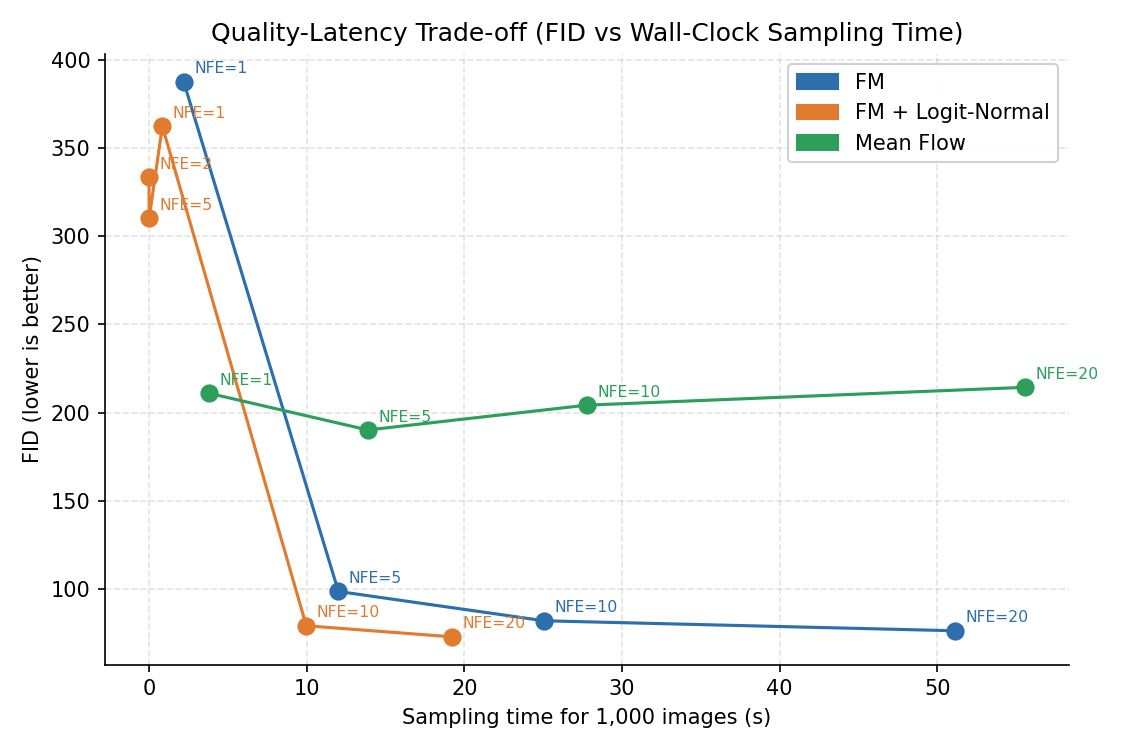
\includegraphics[width=.84\textwidth]{quality_latency.png}\caption{Observed quality--latency points; not hardware-normalized.}\label{fig:latency}\end{figure}
\section{Qualitative evidence}
At 20 NFE, FM variants produce recognizable and diverse CIFAR-10-like content; MF remains noisy, agreeing with its metrics.
\begin{figure}[htbp]\centering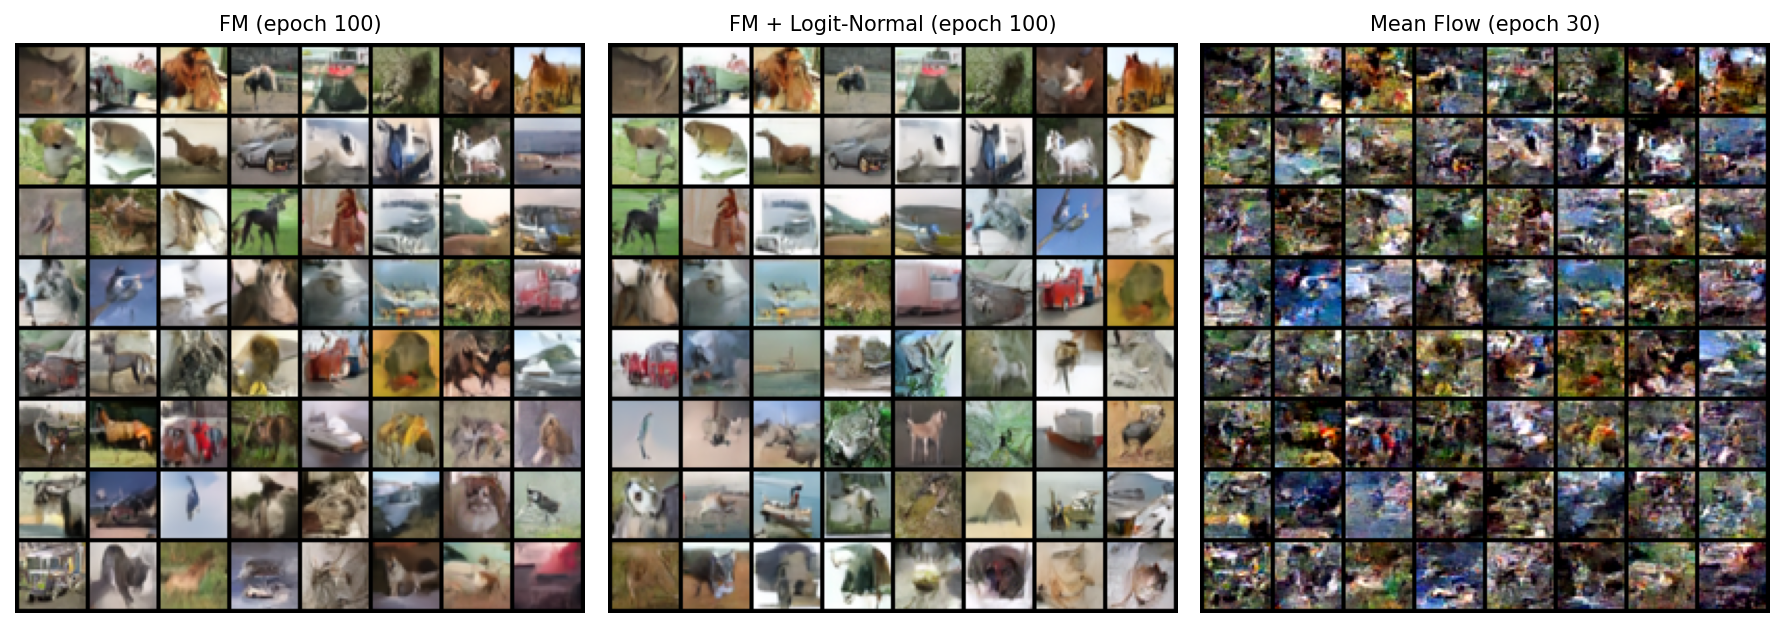
\includegraphics[width=.9\textwidth]{final_samples_nfe20.png}\caption{Fixed-grid final samples at 20 NFE.}\label{fig:samples}\end{figure}
Logit-normal FM has coarse structure by epoch 10 and later refines edges and color. Fixed seed/layout prevents random redraws from masquerading as training progress.
\begin{figure}[htbp]\centering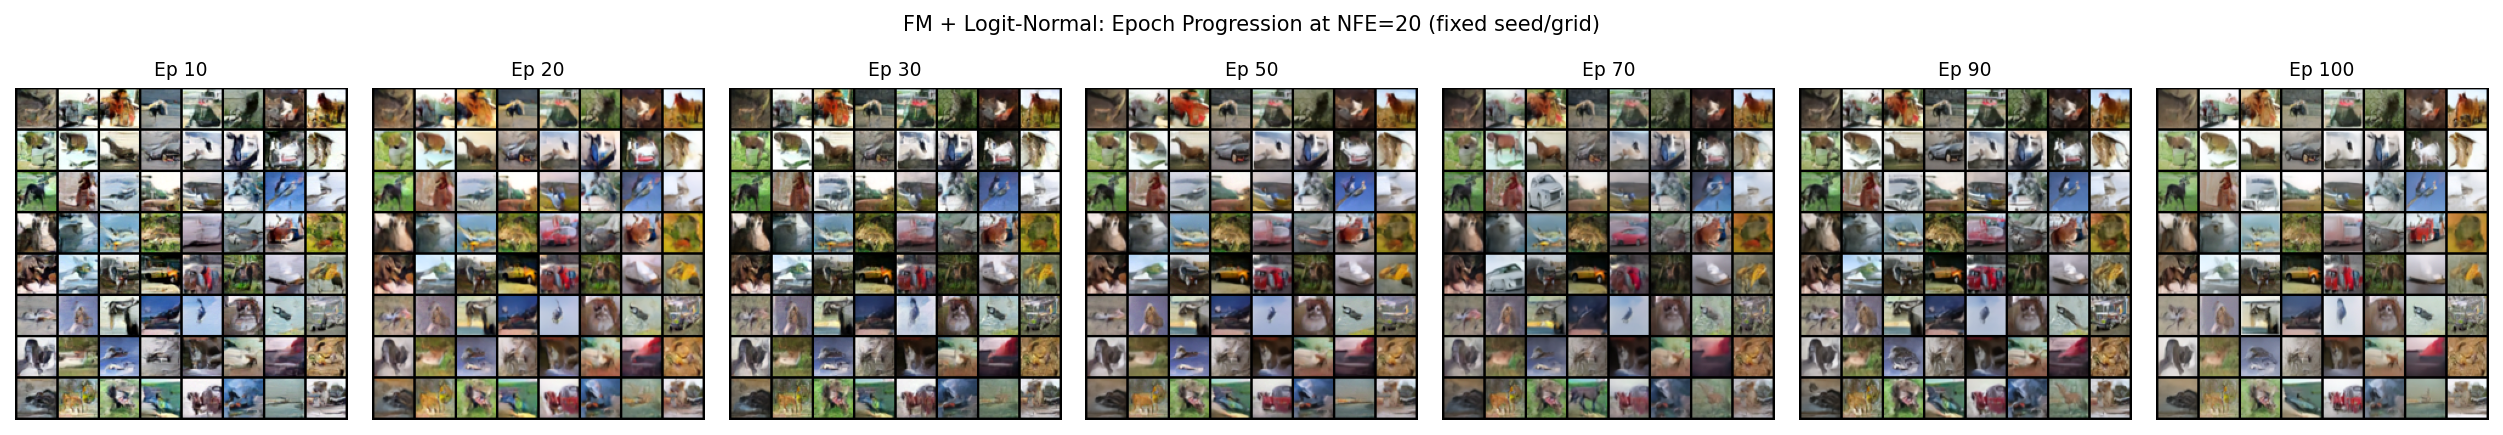
\includegraphics[width=\textwidth]{lognorm_progression.png}\caption{Logit-normal FM progression at fixed NFE and grid positions.}\label{fig:progress}\end{figure}
\begin{figure}[htbp]\centering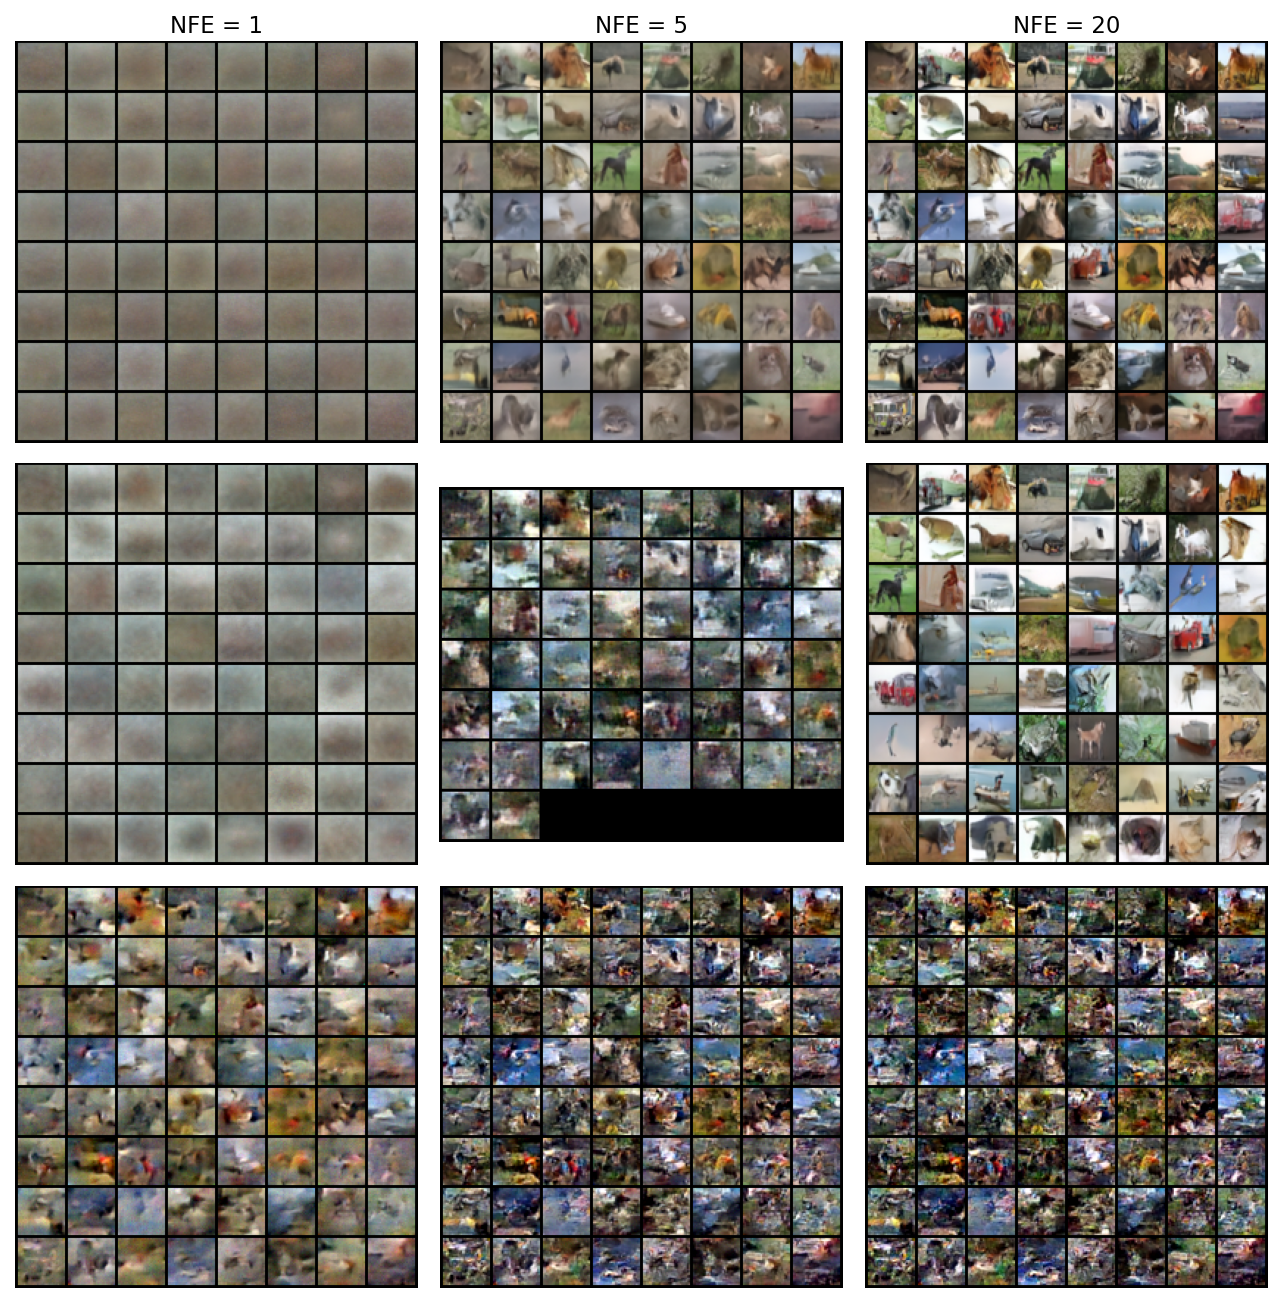
\includegraphics[width=.9\textwidth]{nfe_sample_matrix.png}\caption{Rows are methods; columns show 1, 5, and 20 NFE.}\label{fig:matrix}\end{figure}
\section{Answers to the research questions}
FM variants converge smoothly; MF does not. FM quality improves monotonically with NFE; MF peaks early. Logit-normal FM is the strongest measured multi-step configuration. MF demonstrates one-call mechanics but not competitive quality, and its rising loss identifies training rather than NFE as the bottleneck. Configuration, checkpoint, log, sample, and UI artifacts provide traceability, while public repository traceability awaits the final URL.

\chapter{Challenges and Limitations}
MF's JVP and two-time conditioning increase cost and optimization difficulty. Its 30 epochs, smaller learning rate, additive $r$ conditioning, and absent scheduler may be inadequate. Runs are not compute-matched: batch, steps, epochs, and environment differ. A single seed prevents between-run variance estimation. FID/IS use only 1,000 samples; IS does not compare against real data and neither metric tests memorization. Timing lacks a complete environment fingerprint. MF raw logs include an abandoned 12.5 GB attempt, excluded from the canonical sequence. Checkpoints begin at epoch 10, so no trained images exist for epochs 1--9. Finally, stale README text risks misrepresenting project status.

\chapter{Ethical, Social, and Environmental Considerations}
CIFAR-10 is a small historical web-image benchmark and does not represent the diversity of real deployment settings. Outputs should be labeled synthetic and not described as representative. Low resolution and unconditional generation reduce identity risk, but public extensions still require provenance, a model card, acceptable-use guidance, and data review. This report preserves unfavorable MF results and discloses non-matched budgets rather than overstating success.

Canonical training totals approximately 8.26 GPU-hours, excluding failed attempts, evaluation, and checkpoint generation. Energy/carbon cannot be calculated because power and grid intensity were not logged. Future runs should record GPU model, utilization, power, energy, and location. Before release, local paths and credentials must be removed, documentation updated, licensing added, and large checkpoints hosted appropriately.

\chapter{Conclusion and Future Work}
The project delivers a working and auditable comparison of three flow-based configurations. Logit-normal FM is strongest at 20 NFE (FID 72.66; IS $6.18\pm.52$). Standard FM is close. MF improves the one-step baseline relative to FM but is noisy and its objective rises, showing that an interval displacement is only useful when its average-velocity field is learned accurately. Shared code improves comparability, but rigorous algorithm claims also require matched budgets, seeds, environments, and evaluation counts.

\section{Future direction placeholder}
\fcolorbox{deepblue}{softblue}{\parbox{.88\textwidth}{\textbf{TO BE FINALIZED BY THE TEAM.} Candidate directions: matched-compute multi-seed reruns; Mean Flow sweeps over learning rate and $p_{same}$; stronger joint $(r,t)$ conditioning; EMA and gradient-clipping ablations; 50,000-sample FID with precision/recall and nearest-neighbor checks; higher resolution/class conditioning; and energy instrumentation. Replace with the team-approved scope.}}
\section{Immediate recommendation}
Run at least three seeds under equal examples-seen and equal GPU-hour regimes. Record environment fingerprints, save epoch 0 and early probes, and enlarge evaluation. For MF, first validate the JVP target on an analytic field, then sweep optimization before scaling the backbone.
\printbib

\begin{appendices}
\chapter{Reproducibility and Demonstration}
\begin{lstlisting}[language=bash]
python train.py --config config/fm_full.json --algorithm fm
python train.py --config config/fm_lognorm_rtx3060.json --algorithm fm_lognorm
python train.py --config config/mf_full.json --algorithm mf
python inference_server.py
\end{lstlisting}
Open \texttt{http://localhost:8000}. Demonstrate Train playback, verify checkpoint image/loss synchronization, return Home, open Infer, choose model/NFE/count/seed, generate, then repeat at another NFE. Explain that epoch 0 is noise and epoch 10 the first saved checkpoint.
\chapter{Audit and Artifact Record}
Raw record counts are FM 110 train/12 evaluation/4 sampling; logit-normal FM 100/12/4; MF 59/4/4. Canonical epochs are unique/contiguous; counters increase; losses are finite; parameters are constant; NFE grids are complete. The FM-100 checkpoint stores one module state; MF-30 stores the backbone and four-entry $r$-embedding state. All three load through the inference path.
\small\begin{longtable}{p{.30\textwidth}p{.62\textwidth}}\toprule Artifact&Location\\\midrule\endhead
Metrics&Run-specific \path{metrics/*.jsonl}\\Checkpoints&Run-specific \path{checkpoints/*_epoch*.pt}\\Samples&Run-specific \path{samples/*_nfe*.png}\\Epoch probes&\path{results/checkpoint_samples/fm_lognorm_rtx3060/epoch*.png}\\Demo&\path{index.html}, \path{thesis_dashboard.html}, \path{inference_ui.html}, \path{inference_server.py}\\\bottomrule\end{longtable}\normalsize
\chapter{Submission Placeholders}
\fcolorbox{deepblue}{softblue}{\parbox{.88\textwidth}{\textbf{GITHUB LINK PLACEHOLDER:} Insert final URL and QR code after secret/size/license/documentation checks.}}
\section{Individual contribution}
\begin{longtable}{p{.22\textwidth}p{.52\textwidth}p{.16\textwidth}}\toprule Member&Verified evidence&Share\\\midrule\endhead
Sheikh Mosheul Akbar&TO BE COMPLETED&---\%\\Md. Samiul Islam&TO BE COMPLETED&---\%\\Rad Shahmad Daiyan&TO BE COMPLETED&---\%\\\midrule Total&&100\%\\\bottomrule\end{longtable}
\section{Weekly meetings}
\begin{longtable}{p{.1\textwidth}p{.18\textwidth}p{.22\textwidth}p{.38\textwidth}}\toprule Week&Date&Participants&Verified decisions and actions\\\midrule\endhead
1&TO BE INSERTED&TO BE INSERTED&TO BE INSERTED\\2&TO BE INSERTED&TO BE INSERTED&TO BE INSERTED\\3&TO BE INSERTED&TO BE INSERTED&TO BE INSERTED\\4&TO BE INSERTED&TO BE INSERTED&TO BE INSERTED\\5&TO BE INSERTED&TO BE INSERTED&TO BE INSERTED\\6&TO BE INSERTED&TO BE INSERTED&TO BE INSERTED\\\bottomrule\end{longtable}
\section{Final checklist}
Replace all marked contribution, meeting, GitHub, and future-work placeholders; confirm the defense date and academic designations; update README; rerun the audit after metric changes; exclude data, environments, secrets, and oversized files from the public archive; and inspect a physical print for margins, figure legibility, wrapping, numbering, and signature space.
\end{appendices}
\end{document}
